% !TEX root = D:\Users\Ignacio\Documentos\Escuela\CC3002 - Metodologías de Diseño y Programación\apunte-y-ejercicios\src\latex\Apunte.tex
\section{Herencia}

  En las secciones anteriores dimos una definición para un punto en 2 dimensiones, pero un 
  punto en un plano es algo bastante limitado.
  En esta sección tomaremos la definición inicial de nuestro punto y la generalizaremos 
  para luego, en base a nuestra nueva definición, crear casos más específicos.

  Consideren un vector como una línea que va desde el origen del sistema de coordenadas 
  hasta un punto.
  Un vector en un espacio euclídeo de dimensión \(n\) es una n-tupla de números reales.
  Dada esta definición podemos definir una clase \texttt{VectorND} de la siguiente 
  forma:\footnote{
    La implementación en \textit{Python} la pueden encontrar 
    \href{https://github.com/CC3002-Metodologias/apunte-y-ejercicios/blob/master/src/main/python/vectors.py}{aquí}
  }
  
  \begin{listing}[ht!]
    \begin{minted}{java}
      class VectorND {
        double[] tail;
        
        VectorND(double[] tail) {
          this.tail = tail;
        }
      }
    \end{minted}
  \end{listing}

  Ahora, una característica de los vectores es que pueden sumarse entre ellos.
  La suma de dos vectores es sólo la suma de sus coordenadas, teniendo en cuenta las 
  dimensiones de estos (un vector de \(m\) dimensiones, con \(m \leq n\) es un vector de 
  \(n\) dimensiones en el que todas las componentes \(\mathbf{v}_i\) para \(i > m\) son 
  0).

  \begin{minted}{java}
    VectorND add(VectorND otherVector) {
      double[] bigger, smaller;
      if (tail.length > otherVector.tail.length) {
        bigger = tail;
        smaller = otherVector.tail;
      } else {
        bigger = otherVector.tail;
        smaller = tail;
      }
      double[] components = new double[bigger.length];
      for (int i = 0; i < smaller.length; i++) {
        components[i] = bigger[i] + smaller[i];
      }
      for (int i = smaller.length; i < bigger.length; i++) {
        components[i] = bigger[i];
      }
      return new VectorND(components);
    }
  \end{minted}

  Definamos además un método \texttt{print} que imprima el vector de la forma \((x_0, x_1, 
  ..., x_{n - 1})\).

  
  \begin{minted}{java}
    void print() {
      String result = "(";
      for (int idx = 0; idx < tail.length; idx++) {
        result += tail[idx];
        if (idx < tail.length - 1) {
          result += ", ";
        }
      }
      System.out.println(result + ")");
    }
  \end{minted}
  
  Ahora, es poco común trabajar con vectores de \(n\) dimensiones, en general trabajaremos
  con vectores de dos o tres dimensiones, así que sería una buena idea tener clases 
  específicas para dichos tipos.
  Ahora, ?`Por qué es una buena idea?

  Como mencionamos en el capítulo \ref{ch:oop}, el objetivo de la herencia es la 
  \textbf{especialización} de una clase, y eso es precisamente lo que queremos hacer aquí.
  Tomar un vector de \(n\) dimensiones y crear casos específicos para otros con 
  dimensiones fijas (que tendrán propiedades propias de acuerdo a sus dimensiones).

  Cambiemos el nombre de nuestra clase \texttt{Vector2D} por \texttt{Vector2D} y hagamos
  que sea una subclase de \texttt{VectorND}.

  En \textit{Python}, esto se haría de la siguiente forma:

  \begin{minted}{python}
    class Vector2D(VectorND):
        def __init__(self, x, y):
            super().__init__([x, y])
  \end{minted}

  Aquí, la clase entre paréntesis es la superclase de \texttt{Vector2D}.
  La línea \mintinline{python}{super().__init__([x, y])} lo que hace es llamar al 
  constructor de la superclase (\texttt{VectorND}) y crear un objeto de tipo 
  \texttt{Vector2D} con la lista que se le entregan como parámetros.

  En el caso de \textit{Java}, la herencia se define con la \textit{keyword} 
  \mintinline{java}{extends} de la siguiente forma:

  \begin{minted}{java}
    class Vector2D extends VectorND {

      Vector2D(double x, double y) {
        super(new double[] {x, y});
      }
    }
  \end{minted}

  Como pueden ver, la sintaxis con la que se llama al constructor de la superclase es 
  similar a la manera en la que se hace en \textit{Python}.

  Ahora, los métodos \texttt{add} y \texttt{print} que habíamos definido anteriormente en 
  nuestra clase \texttt{Point2D} ya no son necesarios.
  ?`Por qué pasa esto?
  La explicación la dimos en el capítulo \ref{ch:oop}, ahí dijimos que los hijos heredan 
  sus funcionalidades de su padre, así que si borramos el método \texttt{add} de nuestra
  clase \texttt{Vector2D}, entonces se llamará al método de la superclase.
  Entonces, deberíamos poder ejecutar estos métodos de la misma forma que habíamos hecho 
  antes en la sección \ref{sec:methods} y obtener el mismo resultado.

  \begin{minted}{java}
    Vector2D point = new Vector2D(1, 3);
    Vector2D newPoint = point.add(new Vector2D(-1, 2));
    newPoint.print();
  \end{minted}

  Si intentan correr el código anterior se darán cuenta que no compila.
  ?`Qué hicimos mal?
  El problema es que definimos \texttt{newPoint} como un objeto de tipo \texttt{Vector2D}
  pero el método \texttt{add} retorna un objeto de tipo \texttt{VectorND}.
  Siguiendo esa misma lógica podríamos pensar que hacer 
  \mintinline{java}{point.add(new Vector2D(-1, 2))} también debiera fallar ya que el 
  método espera recibir un objeto de tipo \texttt{VectorND} pero le pasamos uno de tipo
  \texttt{Vector2D}, pero como veremos a continuación ese no es el caso.

  \begin{minted}{java}
    Vector2D point = new Vector2D(1, 3);
    VectorND newPoint = point.add(new Vector2D(-1, 2));
    newPoint.print();
  \end{minted}

  Este código compila y retorna el resultado esperado.
  Ahora, veamos por qué al método \texttt{add} podemos pasarle un parámetro de tipo 
  \texttt{Vector2D} pero no podemos definir \texttt{newPoint} como instancia de esa clase.
  La explicación es simple, \texttt{Vector2D} es más específico que \texttt{VectorND}.
  
  Podemos pensar las clases como conjuntos.
  Sean \(\mathcal{C}_0,\, \mathcal{C}_1\) y \(\mathcal{C}_2\) clases tales que 
  \(\mathcal{C}_1\) y \(\mathcal{C}_2\) heredan de \(\mathcal{C}_0\).
  Esto quiere decir que 

  \[
    \mathcal{C}_0 \subseteq \mathcal{C}_1 \wedge \mathcal{C}_0 \subseteq \mathcal{C}_2
      \implies \mathcal{C}_1 \cap \mathcal{C}_2 \equiv \mathcal{C}_0
  \]
  
  Note que lo anterior implica que para cualquier propiedad \(p \in \mathcal{C}_0\), 
  entonces \(p \in \mathcal{C}_1 \wedge p \in \mathcal{C}_2\), por lo que sabemos que un 
  objeto de tipo \(\mathcal{C}_1\) tiene \textit{al menos} todas las propiedades de 
  \(\mathcal{C}_0\), entonces podemos utilizar un objeto de tipo \texttt{Vector2D} en el 
  método \texttt{add(VectorND)}, ya que sabemos que \texttt{Vector2D} puede 
  hacer todo lo que hace \texttt{VectorND}, esta propiedad se llama \textit{polimorfismo}
  y fue presentada en la sección \ref{sec:objects}.

  Ahora, esto no se da en la dirección contraria. 
  Si tenemos una propiedad \(q \in \mathcal{C}_1\), esta puede o no estar en 
  \(\mathcal{C}_2\).
  Es más, 
  
  \[  q \in \mathcal{C}_1 \wedge q \in \mathcal{C}_2 \iff q \in \mathcal{C}_0.  \]
  
  De esto se desprende que si tenemos un objeto \(o\) de tipo \(\mathcal{C}_0\), dado que 
  anteriormente mostramos que \(\mathcal{C}_1 \cap \mathcal{C}_2 \equiv \mathcal{C}_0\), 
  tenemos \(o \in \{\mathcal{C}_0, \mathcal{C}_1, \mathcal{C}_2\}\).
  Como no podemos distinguir a cuál de esos conjuntos pertenece \(o\), sólo podemos asumir
  que pertenece a la intersección de todos los conjuntos, i.e. \(\mathcal{C}_0\).
  De esto podemos concluir directamente que \texttt{newPoint} puede ser de tipo 
  \texttt{VectorND}, pero no de tipo \texttt{Vector2D}.

  \begin{figure}[ht!]
    \centering
    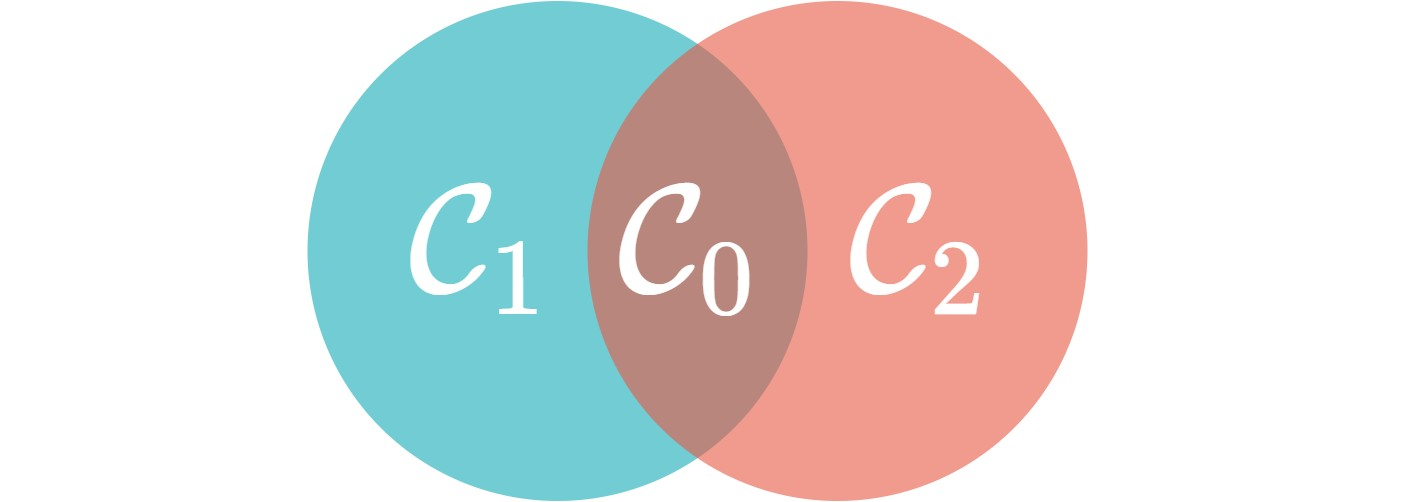
\includegraphics[width=\textwidth]{Inheritance Venn.jpg}
    \caption{Representación de herencia de clases como conjuntos.}  
  \end{figure}

  \begin{note}
    Un detalle que vale la pena mencionar es que \textbf{todos los objetos}, tanto en 
    \textit{Python} como \textit{Java}, extienden implícitamente a un objeto especial 
    llamado \texttt{object} en \textit{Python} y \texttt{Object} en \textit{Java}.
    Así, la definición de la clase \texttt{VectorND} podría hacerse como 
    \mintinline{java}{class VectorND extends Object {...}} y sería equivalente 
    (en \textit{Python} es análogo).
  \end{note}

  \begin{exercise}
    Cree una clase \texttt{Vector3D} que extienda de \texttt{VectorND} e implemente el 
    método \mintinline{java}{void printSpherical()} que imprima en pantalla el vector en 
    coordenadas esféricas de la forma \((r, \phi, \theta)\) sabiendo que:
    
    \[
      \begin{aligned}
        r       &= \sqrt{x^2 + y^2 + z^2} \\
        \phi    &= \arctan{\frac{y}{x}}   \\
        \theta  &= \arccos{\frac{z}{r}}
      \end{aligned}
    \]

    Para esto puede utilizar los métodos de la librería estándar de \textit{Java} 
    \mintinline{java}{Math.sqrt(double)}, \mintinline{java}{Math.atan(double)} y 
    \mintinline{java}{Math.acos(double)}.
  \end{exercise}
%